\documentclass{beamer}
\usepackage{amsmath}
\usepackage{amssymb}
\usepackage{amsthm}                                        
\usepackage{textcomp}     
\usepackage{xcolor}
\usepackage{listings} 
\usetheme{Madrid}
\title{Quaternion Convolutional Neural Network for
Color Image Classification and Forensics}
\author{QILIN YIN\and JINWEI WANG \and  XIANGYANG LUO\and JIANGTAO ZHAI \and SUNIL KR. JHA \and AND YUN-QING SHI}
\date{\today}
\begin{document}
\begin{frame}
    \titlepage
\end{frame}
\begin{frame}
    \begin{figure}[H]
        \centering
        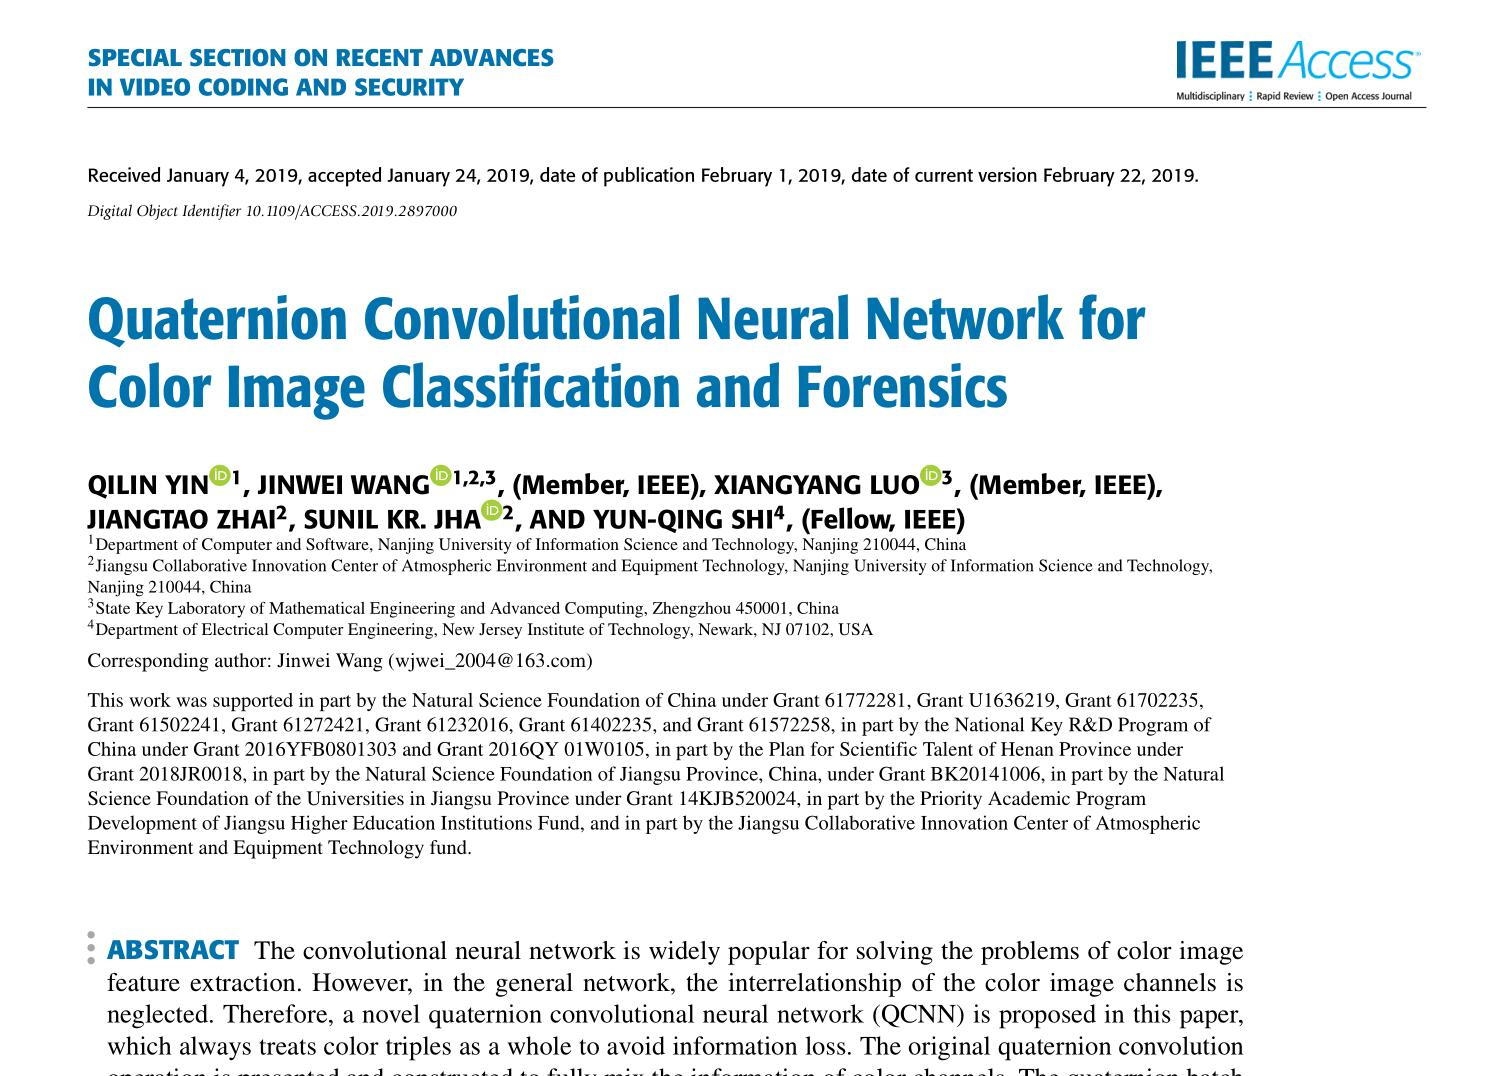
\includegraphics[width=\textwidth]{img/1.jpg}
    \end{figure}
\end{frame}
\begin{frame}
    \frametitle{Table of Content}
    \tableofcontents
\end{frame}
\section{Introduction}
\begin{frame}
    \frametitle{Introduction}
A traditional convolutional neural network consists of one or several convolutional layers, followed by some fully-connected layers of neurons. Each convolution block usually produces feature maps by four steps, e.g.,\textbf{convolution}, \textbf{batch normalization}, \textbf{non-linear activation}, and \textbf{pooling}.
\\~\\
In the last two years, attention model has been widely used in various types of deep learning tasks such as natural language processing, computer vision and speech recognition. From the naming of attention model, it is obvious that it borrows from the human vision attention mechanism. Human vision rapidly focuses on the target area by scanning the global image, and then invests more attention to obtain more detailed information of the target and suppress useless information. Just like this, through the attention model, the neural network can autonomously and purposefully select key features and discard redundant features.
\end{frame}

\begin{frame}
    \frametitle{Introduction}
The traditional CNN framework is becoming more and more mature, but it still has some drawbacks, like when dealing with the color images, general CNNs just treat the RGB three channels as three unrelated feature maps. Although during the convolution process, per convolution kernel sum up the convolution result of different channels as a single output, this still neglects the interrelationship of the RGB three color channels, resulting in the loss of feature information.
\end{frame}

\begin{frame}
    \frametitle{Introduction}
We propose a quaternion convolutional neural network (QCNN) model. a color image can be represented as a quaternion
matrix, each element of which is a pure quaternion consisting of 3-tuple (RGB or LMS). The advantage of this method is that a color can be processed as a hypercomplex number, rather than three separate channels, reserving the interrelationship information between the color channels mostly. So, a color image is circulated and processed in the form of a quaternion matrix in the QCNN. Compared with the traditional CNNs, QCNN not only preserves the vertical relationship between the features, but also maintains the horizontal relationship of the color channels.
\end{frame}

\begin{frame}
    \frametitle{Introduction}
The essence of attention mechanism is to reuse feature maps, give new weight to feature maps and mark out key features. Regardless of the real domain or hypercomplex, this idea is universal. We try to incorporate an attention mechanism into the QCNN model to improve the proposed model performance further. The following experimental results show that our model can outperform the traditional CNN model and the other QCNN model, which has only recently been proposed and is called Pure QCNN by us below.
\end{frame}


\section{Quatrnion Algebra}
\begin{frame}
    \frametitle{Quatrnion Algebra}
A quaternion can be defined as:
$$q=a+bi+cj+dk$$
where $a,b,c,d\in \mathbb{R}$, and the imaginary units $i,j,k$ obey the quaternion rules that $i^2=j^2=k^2=ijk=-1$.If $a = 0$, we can call $q$ is a pure quaternion.
\end{frame}

\begin{frame}
    \frametitle{Quatrnion Algebra}
    \begin{itemize}
        \item Addition:
        \begin{equation*}
            \begin{split}
                q_1+q_2=(a_1+a_2)+(b_1+b_2)i+(c_1+c_2)j+(d_1+d_2)k
            \end{split}
        \end{equation*}
        \item Norm: $$|q|=\sqrt{qq^*}=\sqrt{a^2+b^2+c^+d^2}$$
        \item Conjugation: $$q^*=a-bi-cj-dk$$
        \item Quaternion multiplication: 
        \begin{equation*}
            \begin{split}
                q_1q_2=&(a_1a_2-b_1b_2-c_1c_2-d_1d_2)\\
                            +&(a_1b_2+b_1a_2+c_1d_2-d_1c_2)i\\
                            +&(a_1c_2-b_1d_2+c_1a_2+d_1b_2)j\\
                            +&(a_1d_2+b_1c_2-c_1b_2+d_1a_2)k
            \end{split}
        \end{equation*}
    \end{itemize}
\end{frame}
\section{Components of Quaternion CNN}
\subsection{Quaternion Convolution}
\begin{frame}{Components of Quaternion CNN}{Quaternion Convolution}
Let $W=A+Bi+Cj+Dk$ be a quaternion convolution kernel matrix, and $X=a+bi+cj+dk$ the quaternion input matrix. When a color image is involved, the real part $a$ is set to $0$, and the input matrix becomes the pure quaternion matrix.Similar to the traditional convolution, the quaternion-valued convolution $W\otimes X$ can be defined as follows:
\begin{equation}
    \begin{split}
        W\otimes X=&(Aa-Bb-Cc-Dd)\\
                    +&(Ab+Ba+Cd-Dc)i\\
                    +&(Ac-Bd+Ca+Db)j\\
                    +&(Ad+Bc-Cb+Da)k
    \end{split}
\end{equation}
\end{frame}

% \begin{frame}{Components of Quaternion CNN}{Quaternion Convolution}
%     \begin{figure}[H]
%         \centering
%         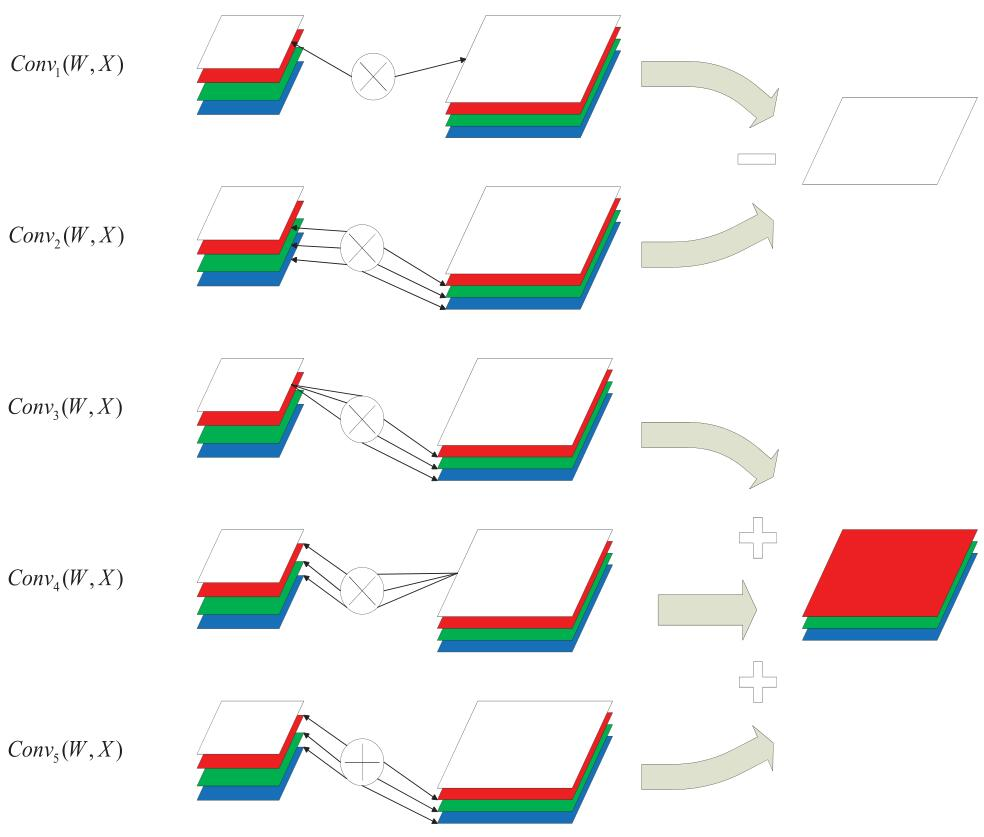
\includegraphics[width=0.7\textwidth]{img/2.jpg}
%         \caption{Real-valued CNN}
%     \end{figure}
%     \end{frame}

% \begin{frame}{Components of Quaternion CNN}{Quaternion Convolution}
% The operator $\otimes$  denotes the normal convolution of two real-valued matrix. The operator $\oplus$ denotes a special convolution that the cross product is used to make the data correspond and convolve. In $Conv_1$ and $Conv_2$, each part of kernel convolve with each part of input correspondingly and separately. The result of real part subtracts the result of three imaginary parts, becoming the real component of the final quaternion. In $Conv_3$, real part of kernel convolve with three imaginary parts of input separately. In Conv4, real part of input convolve with three imaginary parts of kernel separately. In $Conv_5$, three imaginary parts of kernel and input are convolved in a special way that six matrices are paired by the cross product of vectors to produce six conventional convolution. The sum of the result of $Conv_3$, $Conv_4$ and $Conv_5$ yields the imaginary part of final quaternion.
% \end{frame}

\begin{frame}{Components of Quaternion CNN}{Quaternion Batch Normalization}
The quaternion mean and variance have been defined as follows.
\begin{equation}
    \begin{split}
        QE(x)=&\frac{1}{T}\sum_{i=1}^T q_0+q_1i+q_2j+q_3k\\
            =& \overline{q_0} +\overline{q_1} i+\overline{q_2} j+\overline{q_3} k\\
        QV(x)=&\frac{1}{T}\sum_{i=1}^T(x-QE(x))(x-QE(x))^*\\
            =&\frac{1}{T}\sum_{i=1}^T(\Delta q_0^2+\Delta q_1^2+\Delta q_2^2+\Delta q_3^2)\\
    \end{split}
\end{equation}
where $x=q_0+q_1i+q_2j+q_3k, \Delta q_i =q_i-\overline{q_i} $ 
\end{frame}

\begin{frame}{Components of Quaternion CNN}{Quaternion Batch Normalization}
The quaternion batch normalization $QBN(x_i)$ can be defined as:
\begin{equation}
    \begin{split}
        QBN(x_i)=&\gamma(\frac{x_i-QE(x)}{\sqrt{QV(x)+\epsilon}})+\beta\\
            =&\gamma(\frac{q_0^i-\overline{q_0}}{\sqrt{QV(X)+\epsilon}}+\frac{(q_1^i-\overline{q_1})i}{\sqrt{QV(X)+\epsilon}}\\
                &+\frac{(q_2^i-\overline{q_2})i}{\sqrt{QV(X)+\epsilon}}+\frac{(q_3^i-\overline{q_3})i}{\sqrt{QV(X)+\epsilon}})\\
                &+(\beta_0+\beta_1i+\beta_2j+\beta_3k)
    \end{split}
\end{equation}
Here, $\gamma$ is a scalar that initializes to 1, representing stretch
scale, $\beta$ is a quaternion that initializes to 0, representing
shift scale, $\epsilon$ is a non-zero minimum. $\gamma$ and $\beta$ are trainable parameters that participate in network weight updates.
\end{frame}

\subsection{Quaternion Pooling}
\begin{frame}{Components of Quaternion CNN}{Quaternion Pooling}
There are many types of pooling layers, e.g., Max-pooling and Mean-pooling, in the real-valued neural network. They all can be extended to hypercomplex domain. For the Mean-pooling operation, pooling the real part and three imaginary parts of the quaternion matrix separately will not affect final pooling result. 
\\~\\
However, in terms of Max-pooling, if we pool
each part individually, this will create a data mess. Because
we cannot make sure the position of the maximum of each
part is each part is corresponding, we can use some algorithms
to get the guidance matrix for the quaternion matrix. Then,
according to the max pooling result of the guidance matrix,
the four parts of the quaternion matrix can be simplified.
Combining the four parts, the max pooling of the entire quaternion matrix is completed finally. 
\end{frame}

\begin{frame}{Components of Quaternion CNN}{Quaternion Pooling}
    \begin{figure}[H]
        \centering
        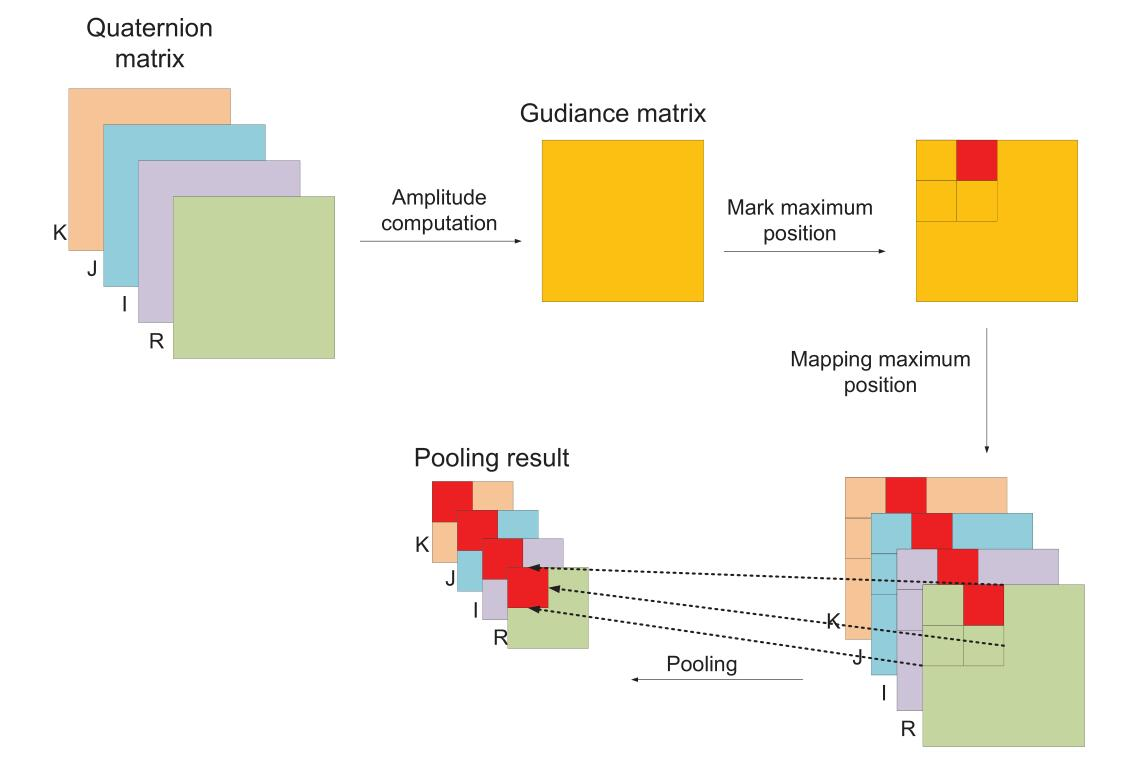
\includegraphics[width=0.8\textwidth]{img/3.jpg}
    \end{figure}
\end{frame}

\subsection{Quaternion Attention Module}
\begin{frame}{Components of Quaternion CNN}{Quaternion Attention Module}
    \begin{figure}[H]
        \centering
        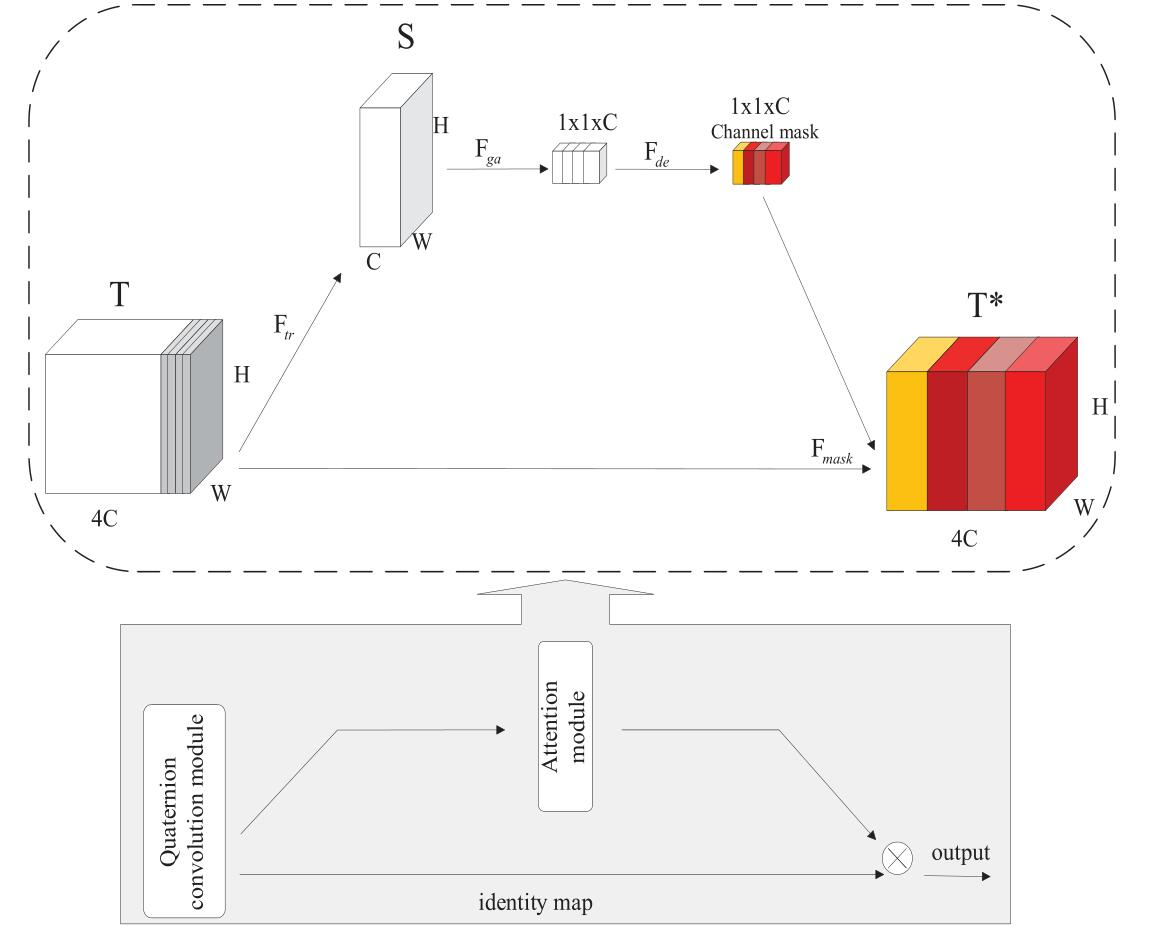
\includegraphics[width=0.7\textwidth]{img/4.jpg}
    \end{figure}
\end{frame}
\begin{frame}{Components of Quaternion CNN}{Quaternion Attention Module}
Let $T\in H\times W\times 4C$ be the input of the quaternion attention module, the number of channel $4C$ shows the uniqueness of the proposed quaternion network too. Because of the
characteristic, we need to modify the attention module in the
general network accordingly to accommodate the data format
of a quaternion. Firstly, $T$ is transformed by an operation $F_{tr}$ to generate guidance data $S\in H\times W\times C$. When it
comes to compressing quaternion data, the transformation
features of quaternion provide us different choices just like
what we do with the quaternion pooling operation. Secondly, $S$ is pooled by a global average pooling $F_{ga}(.)$ to estimate
statistical characteristics of each channel distribution. This
process can be formulated as
\begin{equation}
    z=\frac{1}{H\times W}\sum_{j=1}^H\sum_{i=1}^W S(i,j), z\in 1\times 1\times C
\end{equation}
\end{frame}
\begin{frame}{Components of Quaternion CNN}{Quaternion Attention Module}
Thirdly, $z$ only represents the channel priority distribution
for a mini-batch sample, which is not applicable to the entire
training set, let alone the test set. Therefore, multiple full connection operations $F_{de}(.)$ should be added to the quaternion
module to train a generalized channel weight mask using a
correlation between channels. This
process can be formulated as 
\begin{equation}
    \widetilde{z} =F_{de}(W,z)=\theta(W_2\sigma(W_1z)), W_1\in \frac{C}{r}\times C, W_2\in C\times \frac{C}{r}
\end{equation}
$W_1z$ is a full connection operation, $\sigma$ is a activation operation that is adopted in Relu activation function, $W_2\sigma(W_1z)$ is
another a full connection operation, $\theta$ is also a activation function, but Sigmoid activation function is chosen. $r$ is a hyperparameter, it determines the proportion of data compression
to reduce the amount of computation. 
\end{frame}

\begin{frame}{Components of Quaternion CNN}{Quaternion Attention Module}
Finally, channel mask $\widetilde{z}$
    is combined with $T$ by operation $F_{mask}(.)$ to highlight beneficial features and inhibit unbeneficial ones. 
    \begin{equation}
        T^*=F_{mask}(\widetilde{z},T)=\widetilde{z}T
    \end{equation}
\end{frame}


\subsection{Typical Nonlinear Layer}
\begin{frame}{Components of Quaternion CNN}{Typical Nonlinear Layer}
\begin{equation}
    \mathbb{F}  (q) = \mathbb{F} (a) + \mathbb{F} (b) i + \mathbb{F} (c) j + \mathbb{F} (d) k
\end{equation}
where $\mathbb{F}$ corresponding to any standard activation function.
\end{frame}

\section{Experiment}
\subsection{Architecture}
\begin{frame}{Experiment}{Architecture}
    \begin{figure}[H]
        \centering
        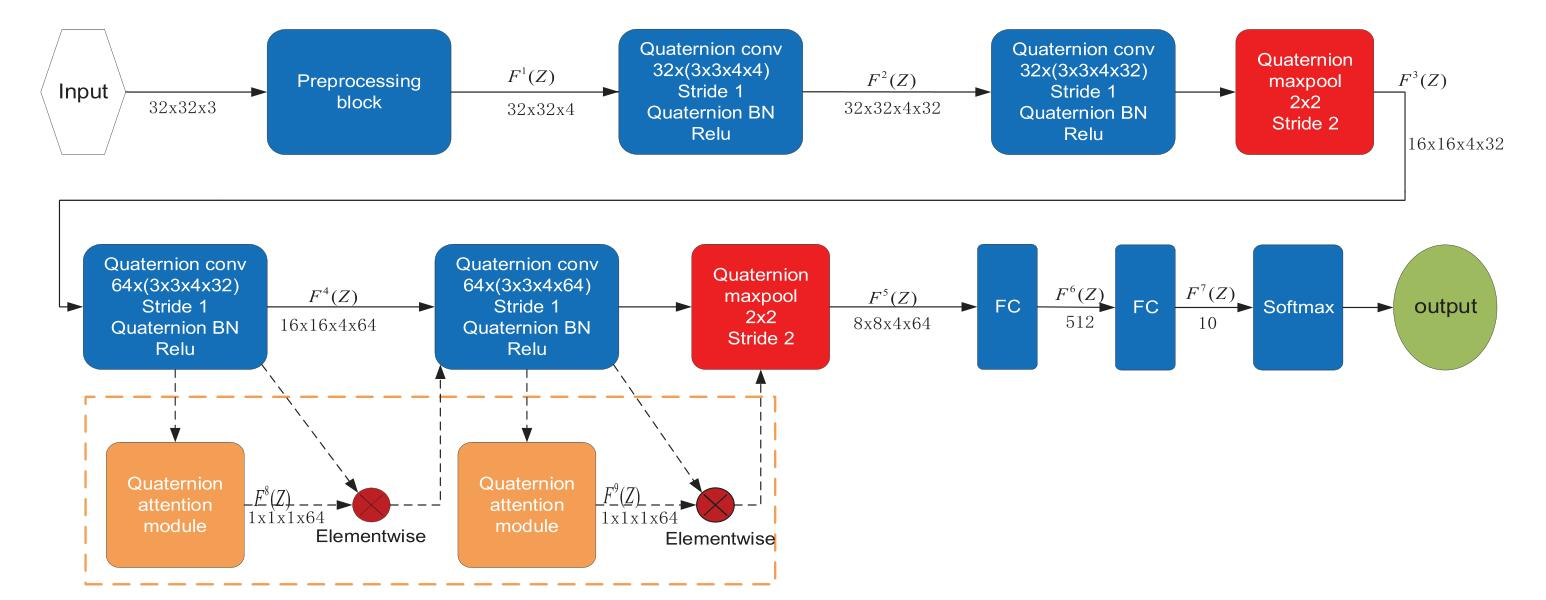
\includegraphics[width=\textwidth]{img/5.jpg}
    \end{figure}
\end{frame}

\begin{frame}{Experiment}{Architecture}
In order to test the performance of the QCNN component
module, we built a basic QCNN. It contains two convolution blocks, two max-pooling layers, and end with two
fully-connected layers. Each convolution block is composed
of two quaternion-valued convolution layers, each of which
contains convolution, batch normalization, and activation
operations. ReLU is used as a standard activation function. Different from traditional convolutional
neural networks, each convolution kernel and feature map
in the proposed model is a quaternion matrix with a size of
$width\times height \times4$. Note that the quaternion attention module
shown in the dotted orange box is not an essential component
of the basic QCNN. It is just a method to improve network
performance.
\end{frame}

\subsection{Rationality of Components}
\subsubsection{Impact of the Quaternion Batch Normalization}
\begin{frame}{Experiment}{Impact of the Quaternion Batch Normalization}
    \begin{figure}[H]
        \centering
        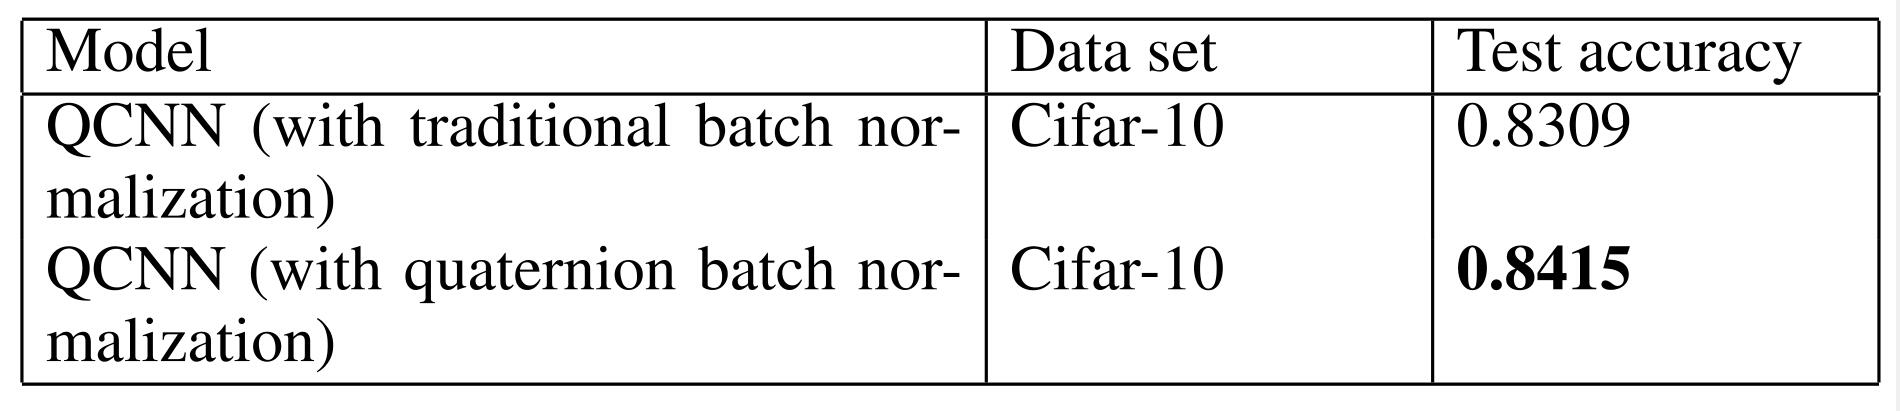
\includegraphics[width=\textwidth]{img/6.jpg}
    \end{figure}
\end{frame}

\subsubsection{Impact of the Quaternion Attention Module}
\begin{frame}{Experiment}{Impact of the Quaternion Attention Module}
    \begin{figure}[H]
        \centering
        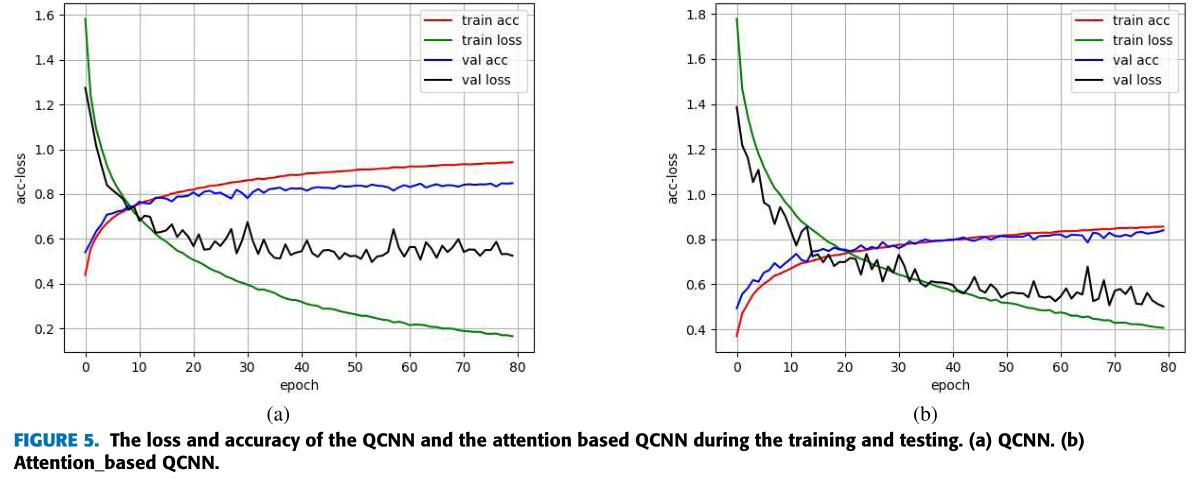
\includegraphics[width=\textwidth]{img/7.jpg}
    \end{figure}
    \begin{figure}[H]
        \centering
        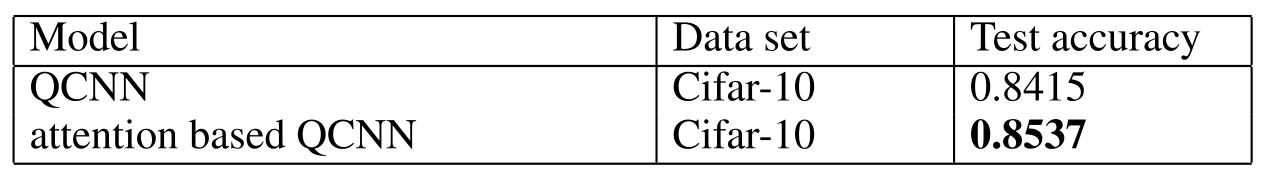
\includegraphics[width=\textwidth]{img/8.jpg}
    \end{figure}
\end{frame}

\subsubsection{Color Image Classification}
\begin{frame}{Experiment}{Color Image Classification}
    \begin{figure}[H]
        \centering
        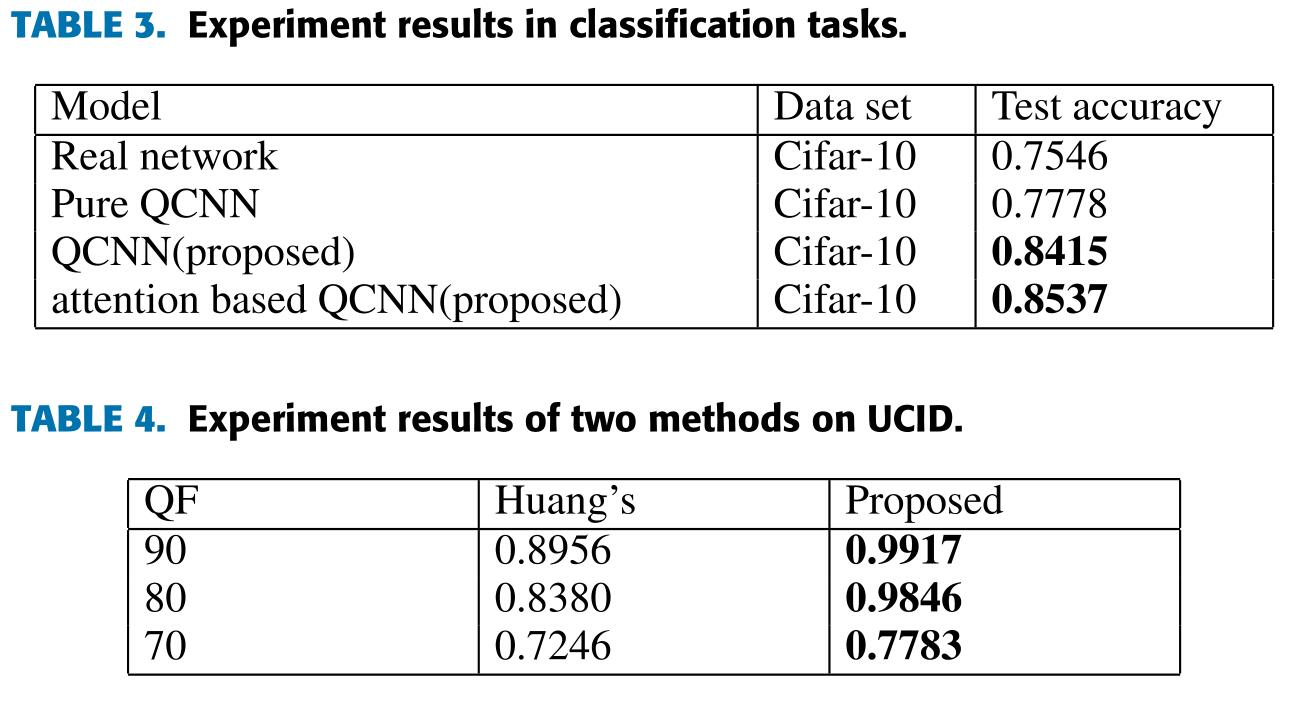
\includegraphics[width=\textwidth]{img/9.jpg}
    \end{figure}
\end{frame}
\end{document}